\documentclass{article}
\usepackage{verbatim}
\usepackage{amsfonts}
\usepackage{geometry}
\usepackage{amsmath}
\usepackage{amsthm}
\usepackage{amssymb}
\usepackage{listings}
\usepackage{graphicx}
\geometry{top=2.5cm,bottom=2.5cm,left=2.5cm,right=2.5cm}
\setlength\parindent{0em}
\begin{document}
\title{Problem Homework(Week 17)}\author{161180162 Xu Zhiming}\maketitle
\large\textbf{CZ: Chapter 4:}\\
\normalsize\textbf{2:}
\begin{proof}
Assume the contrary, that there exist some connected graph $G$ with all its vertices having even degrees, and $G$ has bridges. Suppose one of the bridge in $G$ is between vertices $u$ and $v$. If we remove the bridge, then $G$ becomes disconnected and will consist of two components. $u$ and $v$ belong to different components. The two components are graphs. Besides, $\deg u$ and $\deg v$ are both odd, and the degrees of all other vertices are even, which contradicts the fact that all graphs mustn't have odd number of odd vertices. Therefore, the assumption  is wrong. The thesis is proved.
\end{proof}
\textbf{3:}
\begin{proof}
Suppose the contrary, that there exist another $u-v$ path. We denote it as $P'(u,v)$. $P'(u,v)=(u,x_1,\cdots,x_k,v)$ contains at least three vertices. Since this path is different from $P(u,v)$. $u,v\notin V(P')$ as well as $e=uv\notin E(P')$. Therefore, $P'$ together with $e$ will form a cycle $C=(u,x_1,\cdots,x_k,v,u)$, which contradicts the fact that $e$ is a bridge. Thus the assumption is wrong and the thesis is proved.
\end{proof}
\textbf{5:}\\
\textbf{a:}The size is $n-1$.\\
\textbf{b:}The size is $n-k$.\\
\textbf{16:}\\
\textbf{a:}\\
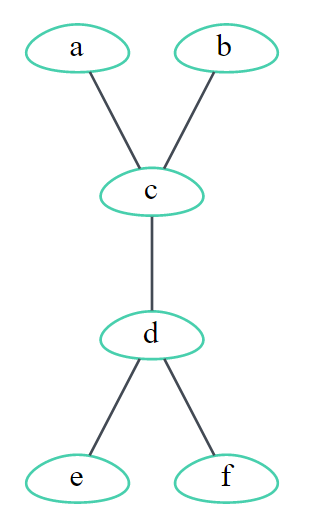
\includegraphics[scale=0.2]{17_1.png}
\textbf{b:}\\
According to the requirements, the order of such a tree $m$ must be a factor of both 3 and 2. That is, $m=6k(k\in N^{+})$. Besides, we have:\\
All vertices' degrees sum:
\begin{equation*}
\begin{aligned}
\frac{2}{3}\cdot 6k+\frac{1}{3}\cdot 6k\cdot 3   
\end{aligned}
\end{equation*}
The number of edges in a tree:
\begin{equation*}
\begin{aligned}
n-1=6k-1
\end{aligned}	
\end{equation*}
Relation between the sum and number of edges:
\begin{equation}
\begin{aligned}
\left(\frac{2}{3}\cdot 6k+\frac{1}{3}\cdot 6k\cdot 3\right)/2=6k-1
\end{aligned}
\end{equation}
From $Equation(1)$, we can solve that $k=1$, which means only the tree with $6$ vertices can have this property and we have drawn it in \textbf{a}.\\
\textbf{17:}
\textbf{a.}\\
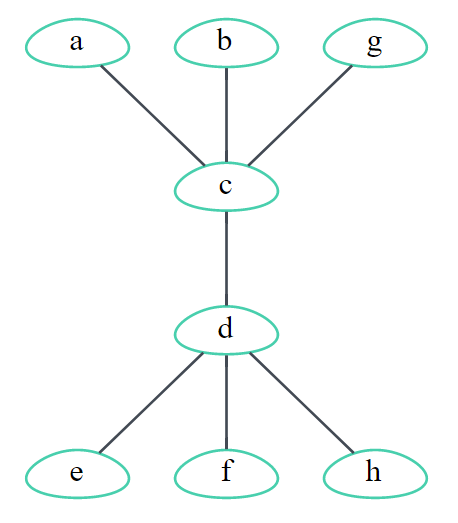
\includegraphics[scale=0.2]{17_2.png}
\textbf{b:}\\
Alike \textbf{4.16(b)}:
\begin{equation}
\begin{aligned}
\left(2k+\frac{2}{3}k\cdot 4\right)/2=\frac{8}{3}k-1
\end{aligned}
\end{equation}
From $Equation(2)$, we can solve that $k=3$, which means only the tree with $8$ vertices can have this property and we have drawn it in \textbf{a}.\\
\textbf{c:}\\
Assume this fixed degree is $f$. Alike in \textbf{b}, we have:
\begin{equation}
\begin{aligned}
\left(2k+\frac{2}{3}k\cdot f\right)/2=\frac{8}{3}k-1
\\k=\frac{3}{5-f},\ k\in N^+,\ f\in N
\end{aligned}
\end{equation}
Therefore:
\begin{equation}
\begin{aligned}
k=2,\ f=4\\
k=1,\ f=2
\end{aligned}
\end{equation}
The solution $k=1,\ f=2$ is obviously impossible, so there exists only one condition drawn in \textbf{a}.\\
\textbf{d:}
Alike before:
\begin{equation}
\begin{aligned}
\left(2k\cdot f+\frac{2}{3}k\right)/2=\frac{8}{3}k-1\\
k=\frac{3}{7-3f},\ k\in N^+,\ f\in N
\end{aligned}
\end{equation}
Therefore:
\begin{equation}
\begin{aligned}
k=3,\ f=2
\end{aligned}
\end{equation}
The graph is drawn below:\\
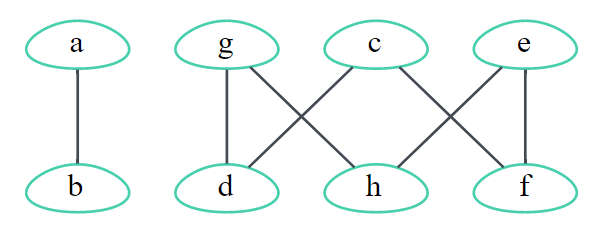
\includegraphics[scale=0.3]{17_3.png}
\textbf{18:}\\
Assume $x$ vertices have degree 3 and $y$ have degree 1, we have:
\begin{equation}
\begin{aligned}
3x+y&=2(n-1)\\
x+y&=n
\end{aligned}
\end{equation}
From $Equation(7)$, $x=(n-2)/2$.\\
\textbf{19:}\\
\textbf{a:}
\begin{proof}
\begin{equation*}
\begin{aligned}
m&=n-1\\
n&=\sum_i^N n_i
2m&=\sum_i^N in_i\\
2\sum_i^N&-2
=\sum_i^N in_i\\
\Rightarrow n_1&=2+n_3+2n_4+4n_6+\cdots
\end{aligned}
\end{equation*}
\end{proof}
\textbf{b:}\\
Number of end-vertices:
\[
\begin{aligned}
n_1&=2+n_3+2n_4\\
&=2+5+2\times 4\\
&=15
\end{aligned}
\]
\textbf{20:}\\
\textbf{a:}
\emph{Disproof:}\\
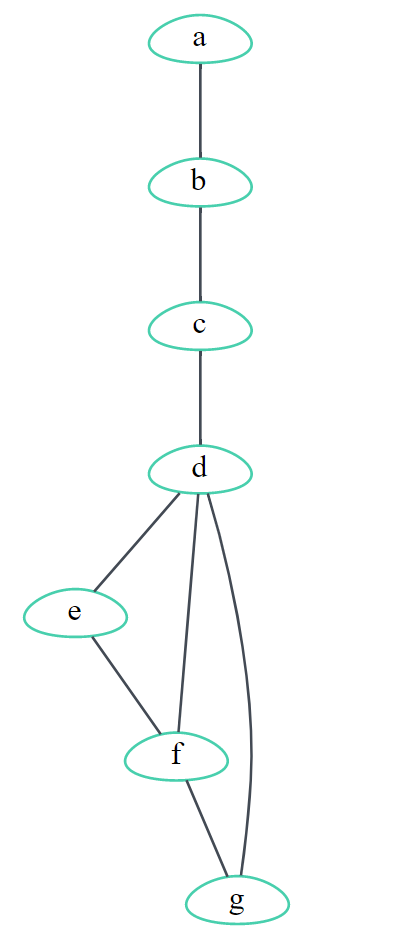
\includegraphics[scale=0.3]{17_4.png}
$n=7,\ m=8.$\\
\textbf{b:}
\begin{proof}
The two regular trees are $K_1$ and $K_2$. For more vertices. Suppose order is $n$ and size is $m$, and the tree is $r-$regular. Then:
\begin{equation*}
\begin{aligned}
\frac{nr}{2}&=m\\
m&=n-1\\
\Rightarrow r&=2-\frac{2}{n}
\end{aligned}
\end{equation*}
$r$ can only equal 1 or 2, leading to $K_1$
and $K_2.$
\end{proof}
\textbf{21:}
\begin{proof}

\end{proof}
\textbf{22:}\\
\[
\begin{aligned}
|E(\bar{T})|=\binom{n}{2}-(n-1)&=\frac{(n-2)(n-1)}{2}=\binom{n-1}{2}\\
|E(K_{n-1})|&=\binom{n-1}{2}\\
Therefore,\\
|E(\bar{T})|&=|E(K_{n-1})|
\end{aligned}
\]
\textbf{23:}\\
Assume the order of $T$ is $n$ and size is $n-1$. Then the order of $\bar{T}$ is also n, and the size is $n-1$. We have:
\[
\begin{aligned}
\binom{n}{2}-(n-1)&=n-1\\
Therefore,\\
n&=4
\end{aligned}
\] 
The sole graph satisfying this property is shown as below:\\
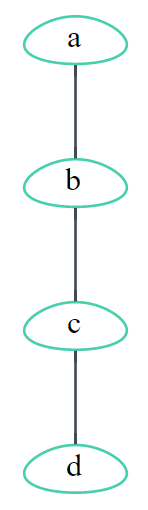
\includegraphics[scale=0.3]{17_5.png}
\end{document}